
\section{Formulation for Implicit Time Steppers for ODEs and DAEs}

\label{rythmos:sec:implicit-time-steppers}

Here we consider several different classes of implicit time stepping
methods. For each class of method we show the set of general nonlinear
equations that defines a single time step and then show how a linearized
form of the equations may be formed to be solved by a Newton-type
nonlinear equation solver.

In particular, for each method, we will show how to define a set of
nonlinear equations of the form 
\begin{equation}
r(z)=0\label{rythmos:eq:r}
\end{equation}
such that when solved will define an implicit time step from $t_{k}$
to $t_{k+1}$, where $\Delta t=t_{k+1}-t_{k}$ denotes the time-step.
In addition, for each method, we will show how to use the DAE residual
evaluation $(\dot{x},x,t){}\rightarrow f$ to define the nonlinear
time step equation (\ref{rythmos:eq:r}). At the highest level, the
time step method only requires very general convergence criteria for
the time step equation (\ref{rythmos:eq:r}) and therefore great flexibility
is allowed in how the time step equation is solved. In general, the
system in (\ref{rythmos:eq:r}) must be solved such that $||x_{k+1}-x^{*}(t_{k+1})||<\eta$,
where $x_{k+1}\in\mathcal{X}$ is the computed step for the state,
$x^{*}(t_{k+1})\in\mathcal{X}$ is the exact state solution at $t_{k+1}$,
and $\eta$ is the maximum allowable local truncation error defined
by the user.

Even though the time step equation can be solved by a variety of means,
a large class of DAEs can also potentially provide support for a general
Newton-type method for solving these equations and can therefore leverage
general software for solving such problems (e.g.\ NOX). The foundation
of Newton-like methods is the ability to solve linear systems similar
to the Newton system 
\begin{equation}
\Jac{r}{z}\Delta z=-r(z_{l})
\end{equation}
where $z_{l}$ is the current candidate solution of the nonlinear
equations (which also defines the point where $\jac{r}{z}$ is evaluated)
and $\Delta z=r_{l+1}-r_{l}$ is the update direction. Line-search
Newton methods then define an update to the solution along the direction
$\Delta z$. The essential functionality needed to perform a Newton-like
method are the the abilities to evaluate the nonlinear residual $z{}\rightarrow r$
and to (approximately) solve linear systems involving the Jacobian
matrix $\jac{r}{z}$. For each type of implicit time integration method,
we will show, if possible, how to perform solves with $\jac{r}{z}$
by performing solves with the matrix 
\begin{equation}
W=\alpha\Jac{f}{\dot{x}}+\beta\Jac{f}{x},\label{rythmos:eq:W}
\end{equation}
evaluated at points $(\dot{x},x,t)$ selected by the time integration
method and where $\alpha\in\RE$ and $\beta\in\RE$ is some constants
also defined by the time integration method. Note that the matrix
$W$ above in (\ref{rythmos:eq:W_bdf}) may not necessarily exactly
represent $\jac{r}{z}$ and $z$ and $r$ may not simply lie in the
vector spaces $\mathcal{X}$ and $\mathcal{F}$ respectively; but
in many cases, they will.

The iteration matrix, $W$, is defined to be
\[
W\equiv\frac{df}{dx_{n}}=\frac{\partial\dot{x}}{\partial x_{n}}\Jac{f}{\dot{x}}+\frac{\partial x}{\partial x_{n}}\Jac{f}{x}=\alpha\Jac{f}{\dot{x}}+\beta\Jac{f}{x}
\]
where $\alpha=\partial\dot{x}/\partial x_{n}$ and $\beta=\partial x/\partial x_{n}$,
and recalling $f\left(\dot{x}(x_{n}),x(x_{n})\right)=0$.


\subsection{Backward Euler}

\begin{figure}[H]
\centering{}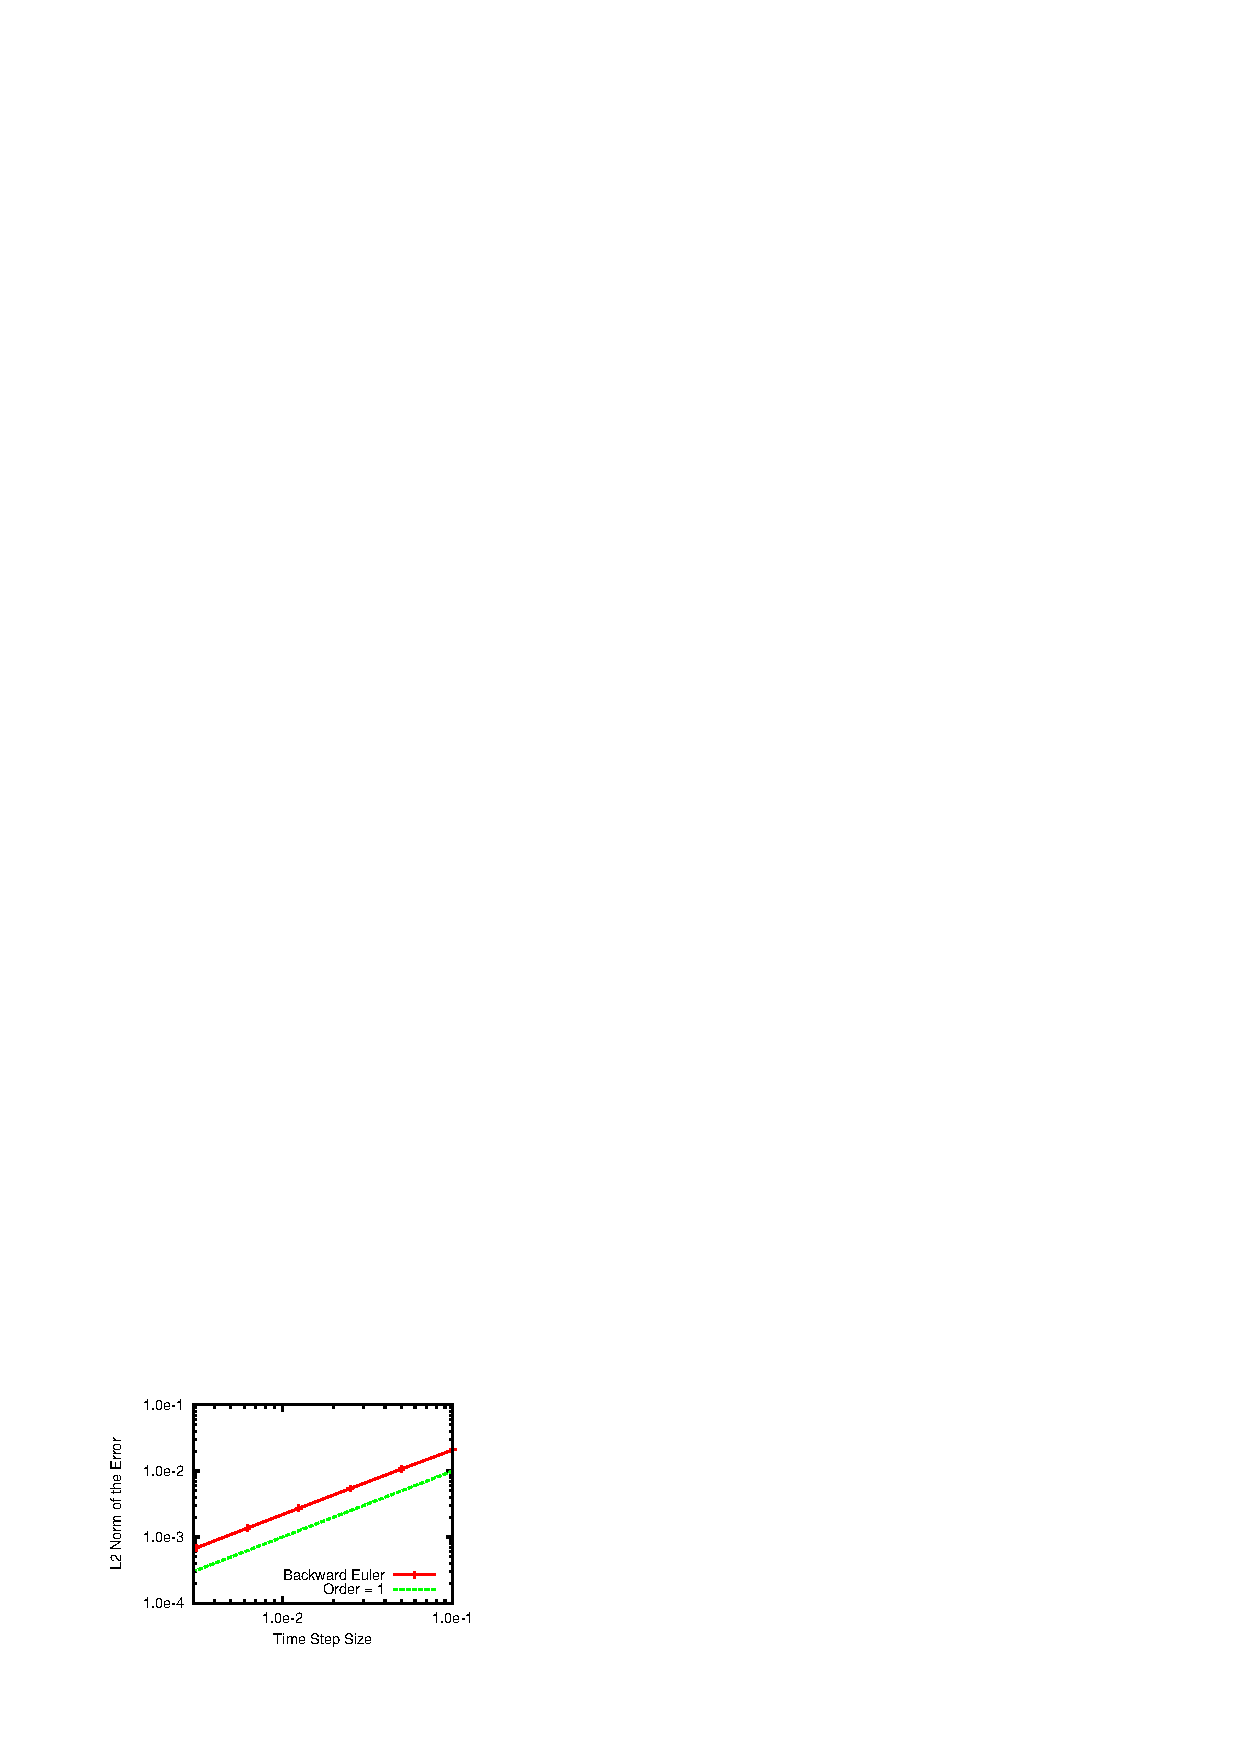
\includegraphics[scale=1.5]{figures/BackwardEuler}\caption{Order of accuracy for the SinCos Problem (Section~\ref{rythmos:sec:SinCos-Problem})
using Backward Euler.}
\end{figure}

